% Options for packages loaded elsewhere
% Options for packages loaded elsewhere
\PassOptionsToPackage{unicode}{hyperref}
\PassOptionsToPackage{hyphens}{url}
\PassOptionsToPackage{dvipsnames,svgnames,x11names}{xcolor}
%
\documentclass[
  12pt,
]{article}
\usepackage{xcolor}
\usepackage[margin=2cm]{geometry}
\usepackage{amsmath,amssymb}
\setcounter{secnumdepth}{-\maxdimen} % remove section numbering
\usepackage{iftex}
\ifPDFTeX
  \usepackage[T1]{fontenc}
  \usepackage[utf8]{inputenc}
  \usepackage{textcomp} % provide euro and other symbols
\else % if luatex or xetex
  \usepackage{unicode-math} % this also loads fontspec
  \defaultfontfeatures{Scale=MatchLowercase}
  \defaultfontfeatures[\rmfamily]{Ligatures=TeX,Scale=1}
\fi
\usepackage{lmodern}
\ifPDFTeX\else
  % xetex/luatex font selection
\fi
% Use upquote if available, for straight quotes in verbatim environments
\IfFileExists{upquote.sty}{\usepackage{upquote}}{}
\IfFileExists{microtype.sty}{% use microtype if available
  \usepackage[]{microtype}
  \UseMicrotypeSet[protrusion]{basicmath} % disable protrusion for tt fonts
}{}
\makeatletter
\@ifundefined{KOMAClassName}{% if non-KOMA class
  \IfFileExists{parskip.sty}{%
    \usepackage{parskip}
  }{% else
    \setlength{\parindent}{0pt}
    \setlength{\parskip}{6pt plus 2pt minus 1pt}}
}{% if KOMA class
  \KOMAoptions{parskip=half}}
\makeatother
% Make \paragraph and \subparagraph free-standing
\makeatletter
\ifx\paragraph\undefined\else
  \let\oldparagraph\paragraph
  \renewcommand{\paragraph}{
    \@ifstar
      \xxxParagraphStar
      \xxxParagraphNoStar
  }
  \newcommand{\xxxParagraphStar}[1]{\oldparagraph*{#1}\mbox{}}
  \newcommand{\xxxParagraphNoStar}[1]{\oldparagraph{#1}\mbox{}}
\fi
\ifx\subparagraph\undefined\else
  \let\oldsubparagraph\subparagraph
  \renewcommand{\subparagraph}{
    \@ifstar
      \xxxSubParagraphStar
      \xxxSubParagraphNoStar
  }
  \newcommand{\xxxSubParagraphStar}[1]{\oldsubparagraph*{#1}\mbox{}}
  \newcommand{\xxxSubParagraphNoStar}[1]{\oldsubparagraph{#1}\mbox{}}
\fi
\makeatother


\usepackage{longtable,booktabs,array}
\usepackage{calc} % for calculating minipage widths
% Correct order of tables after \paragraph or \subparagraph
\usepackage{etoolbox}
\makeatletter
\patchcmd\longtable{\par}{\if@noskipsec\mbox{}\fi\par}{}{}
\makeatother
% Allow footnotes in longtable head/foot
\IfFileExists{footnotehyper.sty}{\usepackage{footnotehyper}}{\usepackage{footnote}}
\makesavenoteenv{longtable}
\usepackage{graphicx}
\makeatletter
\newsavebox\pandoc@box
\newcommand*\pandocbounded[1]{% scales image to fit in text height/width
  \sbox\pandoc@box{#1}%
  \Gscale@div\@tempa{\textheight}{\dimexpr\ht\pandoc@box+\dp\pandoc@box\relax}%
  \Gscale@div\@tempb{\linewidth}{\wd\pandoc@box}%
  \ifdim\@tempb\p@<\@tempa\p@\let\@tempa\@tempb\fi% select the smaller of both
  \ifdim\@tempa\p@<\p@\scalebox{\@tempa}{\usebox\pandoc@box}%
  \else\usebox{\pandoc@box}%
  \fi%
}
% Set default figure placement to htbp
\def\fps@figure{htbp}
\makeatother





\setlength{\emergencystretch}{3em} % prevent overfull lines

\providecommand{\tightlist}{%
  \setlength{\itemsep}{0pt}\setlength{\parskip}{0pt}}



 


\makeatletter
\@ifpackageloaded{caption}{}{\usepackage{caption}}
\AtBeginDocument{%
\ifdefined\contentsname
  \renewcommand*\contentsname{Table of contents}
\else
  \newcommand\contentsname{Table of contents}
\fi
\ifdefined\listfigurename
  \renewcommand*\listfigurename{List of Figures}
\else
  \newcommand\listfigurename{List of Figures}
\fi
\ifdefined\listtablename
  \renewcommand*\listtablename{List of Tables}
\else
  \newcommand\listtablename{List of Tables}
\fi
\ifdefined\figurename
  \renewcommand*\figurename{Figure}
\else
  \newcommand\figurename{Figure}
\fi
\ifdefined\tablename
  \renewcommand*\tablename{Table}
\else
  \newcommand\tablename{Table}
\fi
}
\@ifpackageloaded{float}{}{\usepackage{float}}
\floatstyle{ruled}
\@ifundefined{c@chapter}{\newfloat{codelisting}{h}{lop}}{\newfloat{codelisting}{h}{lop}[chapter]}
\floatname{codelisting}{Listing}
\newcommand*\listoflistings{\listof{codelisting}{List of Listings}}
\makeatother
\makeatletter
\makeatother
\makeatletter
\@ifpackageloaded{caption}{}{\usepackage{caption}}
\@ifpackageloaded{subcaption}{}{\usepackage{subcaption}}
\makeatother
\usepackage{bookmark}
\IfFileExists{xurl.sty}{\usepackage{xurl}}{} % add URL line breaks if available
\urlstyle{same}
\hypersetup{
  pdftitle={Spatial Inequalities in Educational Infrastructure: Bayesian Hierarchical Modelling of School Availability Across North Borneo},
  pdfauthor={Alvin Bong},
  colorlinks=true,
  linkcolor={blue},
  filecolor={Maroon},
  citecolor={Blue},
  urlcolor={Blue},
  pdfcreator={LaTeX via pandoc}}


\title{Spatial Inequalities in Educational Infrastructure: Bayesian
Hierarchical Modelling of School Availability Across North Borneo}
\author{Alvin Bong}
\date{}
\begin{document}
\maketitle
\begin{abstract}
Understanding the spatial distribution of educational infrastructure is
essential for ensuring equitable access to schooling. This study
examines regional disparities in school availability across Brunei and
the neighboring Malaysian states of Sarawak and Sabah, with a focus on
identifying potential underserved areas. First, exploratory data
analysis (EDA) was conducted to compare school counts and
student-teacher ratios at the district level across the three regions.
The core analysis employs Standardized Incidence Ratio (SIR) and
Bayesian spatial Poisson model using Integrated Nested Laplace
Approximation (INLA) to estimate the relative abundance of schools
across Brunei's districts, adjusting for expected counts based on
population, region size and socioeconomic indicator (house price +
partially simulated). Spatially structured and unstructured random
effects were incorporated to account for latent spatial processes.
Posterior estimates identified districts with significantly lower school
availability than the national baseline, supporting future policy
planning and school placement.
\end{abstract}


\subsection{Introduction}\label{introduction}

Education is a foundational pillar of national development and its
people, influencing social well-being, economic growth, and long-term
sustainability. The global significance of education is recognized in
Sustainable Development Goal 4, which promotes inclusive and equitable
quality education for all {[}1{]}. Nationally, Brunei Darussalam's
national vision, Wawasan Brunei 2035, positions education as a
cornerstone of the country's long-term development goals. Ensuring
equitable access to education through sufficient infrastructure, fair
resource distribution, and balanced student--teacher ratios is critical
to delivering quality learning experiences.

While several studies have examined general aspects of education in
Brunei, there have been limited studies based on quantitative spatial
methods, with only one examining the spatial distribution and hotspots
of schools. This project aims to addresses that gap by first conducting
a comparative analysis of school availability and student--teacher
ratios across Brunei's districts, with additional context from
neighboring Malaysian states, Sarawak and Sabah.

Next, Standardized Incidence Ratios (SIR) and Bayesian hierarchical
models are used to identify adminstrative regions in Brunei where school
availability falls significantly below the national baseline, supporting
future policy planning and school placements.

\subsection{Data}\label{data}

This study focuses exclusively on government primary and secondary
schools, as these institutions serve as the main access points to
education for most youth. The school dataset from 2018 was used as it is
the most recent year for which disaggregated school-level data is
available in Brunei. Although more recent statistics exist, they are
published only in summary form.

Population data is drawn from the 2021 national census, the most recent
census available in Brunei, despite the mismatch in years with the
school dataset. Brunei conducts its national census every ten years,
making the 2021 data the best option for population estimates.

The following key data variables were used: school counts,
administrative boundary data, population, student--teacher ratios, and
house prices. These datasets were cleaned, wrangled, and merged
primarily using left\_join() and rbind(), with further details provided
below.

\subsubsection{Brunei}\label{brunei}

Data on school locations, student--teacher ratios, administrative
boundaries, and population were sourced from the \texttt{bruneimap} R
package. The school dataset \texttt{sch\_sf} includes georeferenced
point data for each institution. For our areal analysis, schools were
aggregated by district and mukim (finer administrative level). Despite
composing of only four districts, district-level aggregation was used
for broader comparisons (student--teacher ratios and school counts) to
match the size of available administrative resolution in Malaysian data.
Mukims (\(N = 39\)), which provide finer geographic resolution, were
instead used for the Bayesian spatial analysis of school availability in
Brunei.

To incorporate a socioeconomic indicator, we used median house prices
derived from approximately 30,000 property listings spanning 1993--2025.
These were calculated at the mukim level and included as a covariate in
the Bayesian model. In cases where house price data were missing, values
were imputed using predictions from an INLA-based Gaussian model. Manual
imputations based on local knowledge were initially tested, but the
INLA-predicted values were ultimately adopted, as both methods produced
similar model outcomes. Given the nature of the data, house prices were
treated as partially simulated estimates and may not fully reflect
actual market values.

\subsubsection{Malaysia}\label{malaysia}

Malaysian data variables were sourced from the national open data portal
{[}data.gov.my{]}, and include district-level school counts and
population estimates for the states of Sarawak and Sabah. Administrative
boundary (districts) were obtained via the \texttt{geomdata} R package,
as OpenStreetMap (\texttt{osmdata}) does not provide required
administrative divisions level.

Some inconsistencies were found between school data and adminstrative
boundaries, particularly in areas where older districts had been
subdivided into newer ones. In these cases, school counts were available
only for the original (larger) districts. To ensure consistency, we
excluded the newer subdivisions and manually reassigned schools in the
affected areas to the nearest valid district.

\subsection{Method}\label{sec-method}

Exploratory data anlysis using Clorepath maps for schools count, by area
(usingst\_area) studnet teacher ratio

\subsubsection{Spatial regression model}\label{spatial-regression-model}

Let \(Y_i\) and \(E_i\) denote the observed and expected counts of
schools, respectively, in mukim \(i \in \{1, \dotsc, n\}\). Let
\(\theta_i\) represent the \emph{relative abundance} of schools in mukim
\(i\), analogous to a relative risk in disease mapping. The model is
specified as follow:

\[
Y_i \mid \theta_i \sim \text{Poisson}(E_i \cdot \theta_i), \quad i = 1, \dotsc, n
\]

\[
\log(\theta_i) = \beta_0 + \beta_1 \cdot \text{pop}_i + \beta_2 \cdot \text{area}_i + \beta_3 \cdot \text{hp}_i + u_i + v_i
\]

Where:

\begin{itemize}
\tightlist
\item
  \(\beta_0\) is the intercept,
\item
  \(\beta_1\), \(\beta_2\), and \(\beta_3\) are regression coefficients
  for the standardized covariates:

  \begin{itemize}
  \tightlist
  \item
    \(\text{pop}_i\): population (in units of 10,000),
  \item
    \(\text{area}_i\): mukim size (in units of 10 km²),
  \item
    \(\text{hp}_i\): median house price (in BND \$1,000,000),
  \end{itemize}
\item
  \(u_i\) is a structured spatial effect, modelled using an intrinsic
  conditional autoregressive (CAR) prior
  \(u_i \mid u_{-i} \sim \mathcal{N}(\bar{u}_{\delta_i}, \frac{1}{\tau_u n_{\delta_i}})\)
\item
  \(v_i\) is an unstructured random effect,
  \(v_i \sim \text{Normal}(0, \frac{1}{\tau_v})\)
\end{itemize}

The spatial random effect \(u_i\) requires a neighborhood (adjacency)
matrix. Here, We define two mukims as neighbors if they share at least
one boundary point (Queen contiguity). The neighborhood graph is
constructed using the \texttt{poly2nb()} function from the
\texttt{spdep} package. Model fitting was performed in a Bayesian
framework using the Integrated Nested Laplace Approximation (INLA).

\subsection{Results}\label{sec-results}

\subsubsection{Model}\label{model}

The model results show that the intercept is estimated at
\(\hat{\beta}_0 = 1.077\), with a 95\% credible interval of
\((0.239, 1.894)\). The coefficient for population,
\(\beta_1 = -0.436\), with a 95\% credible interval of
\((-0.579, -0.295)\), indicates a statistically significant negative
relationship between population size and relative school abundance.
Specifically, for every 10,000 increase in population, the relative
abundance of schools decreases by approximately 35\%, since
\(\exp(-0.436) \approx 0.647\). In contrast, the covariates: mukim size
and house price are not statistically significant. The coefficient for
mukim size is \(\hat{\beta_2}=0.015\) (95\% CI: -0.002, 0.032), and for
house price is \(\hat{\beta_3}=-0.759\) (95\% CI: -3.174, 1.704).

The estimated relative abundance (RA) of schools across mukims indicates
lower values in the northern coastal mukims, particularly in northern
Brunei-Muara District, along the South China Sea. Conversely, higher RA
values appear inland, especially in less densely populated regions.

To identify mukims with potentially inadequate school provision,
non-exceedence probabilities were computed for a threshold of
\(RA <0.7\). The analysis indicates that it is highly likely that
several mukims fall below this threshold, including Mukim Sengkurong,
Mukim Gadong A, Mukim Gadong B, Mukim Berakas B, and Mukim Mentiri.

\pandocbounded{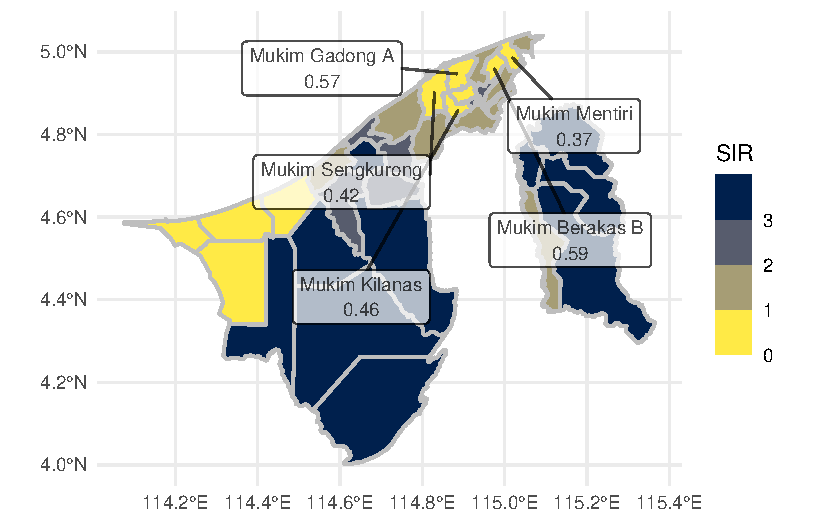
\includegraphics[keepaspectratio]{index_files/figure-pdf/unnamed-chunk-6-1.pdf}}

\pandocbounded{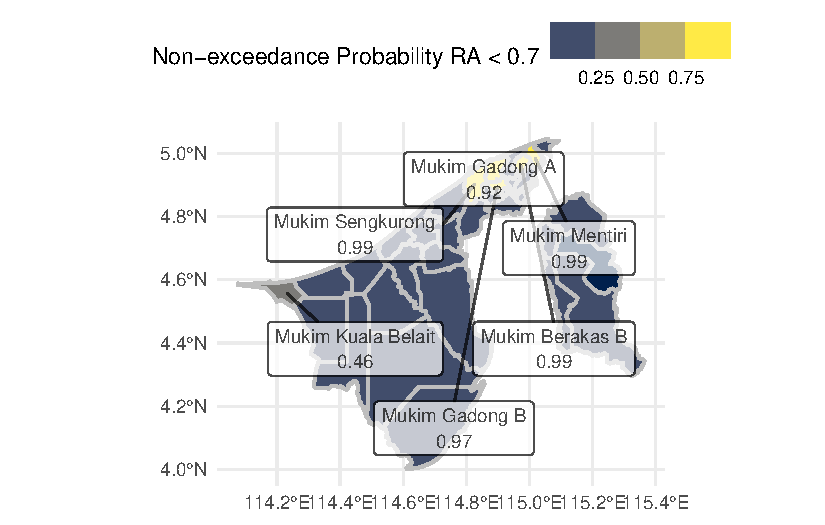
\includegraphics[keepaspectratio]{index_files/figure-pdf/unnamed-chunk-7-1.pdf}}

\subsection{Discussion \& Limitation}\label{discussion-limitation}

The negative relationship between population and school counts, as well
as higher RA values in inland (rural) mukims than coastal ares with
larger population suggests that school availability in rural mukims seem
to be adequate, potentially due to legacy planning policies or
intentional efforts to ensure equitable access in remote areas.

In contrast, urban and peri-urban mukims in the Brunei-Muara District,
the country's most densely populated and economically active region,
show signs of disparities in school access. Notably, the high
non-exceedance probability of \(RA < 0.7\) in \textbf{Mukim Sengkurong,
Gadong A \& B, Berakas B, and Mentiri} indicates that they have fewer
schools than expected relative to their population sizes. These
disparities highlight areas that may be underinvested in educational
infrastructure, warranting closer policy attention.

Importantly, these mukims are also encompass several new government
housing developments, such as Perpindahan Lugu and Perpindahan Tanah
Jambu. This suggests a potential planning gap, where population is
increasing due to housing developments, but educational infrastructure
has not yet caught up.

However, inspection of the Choropleth map of school counts per mukim
reveals that these areas have a similar number of schools compared to
their neighboring mukims. This suggests that while the absolute number
of schools may not be unusually low, the rapid increase in population
within these new housing areas may have outpaced school capacity,
leading to a situation where demand exceeds supply within these specific
zones.

Nevertheless, this situation represents a strategic opportunity.
Prioritizing school construction in these fast-growing neighborhoods
could significantly improve access to education, reduce commute times,
lower transportation costs, and enhance the overall quality of life for
residents. Locating schools closer to homes supports national goals
related to sustainable urban development, walkability, and equity in
public services.

\subsubsection{Limitations}\label{limitations}

This study is limited to public schools, excluding private and
international institutions that may affect school availability in some
areas. The data is from 2018, potentially missing recent changes,
especially in fast-growing neighborhoods. It also does not account for
school types (e.g., primary vs.~secondary) or age-specific population
data, which are important for demand estimation. Housing price was used
as a proxy for socioeconomic status, but data relies on listing prices,
which may not reflect actual market values due to negotiation factors.
In some areas, price data was also simulated, introducing further
uncertainty.

\subsection{Conclusions}\label{sec-conc}

In summary, the analysis reveals a negative relationship between
population size and relative school abundance, suggesting urban areas
have fewer schools per capita than rural ones. Several mukims in the
Brunei-Muara District, including Sengkurong, Gadong A \& B, Berakas B,
and Mentiri, appear to have fewer schools than expected, despite ongoing
population growth driven by new housing developments. While total school
counts may seem adequate, local demand in these areas may exceed
capacity. Addressing this gap offers a strategic opportunity to improve
access, reduce travel time, and support equitable urban planning.

\subsection*{References}\label{references}
\addcontentsline{toc}{subsection}{References}

\phantomsection\label{refs}




\end{document}
